\section{Validation against Hu et al.\ (2017) and Smith et al.\ (2021)}
\label{sec:validation}

\subsection{Setup}

\texttt{examples/SubgridTests/StromgrenSphereClumpSmith2021/} reproduces
both papers' D-type expansion test directly: four co-located
19.2\,M$_\odot$ sources ($\dot N_{\rm ion}\approx2.5\times10^{48}\,
{\rm s^{-1}}$ each, $1\times10^{49}\,{\rm s^{-1}}$ combined), a uniform
$100\,{\rm cm^{-3}}$, $10^3\,$K background, and (for the clump test) a
10\,pc-radius, $10^4\,{\rm cm^{-3}}$ clump 20\,pc from the sources --
all confirmed against the papers' own text, not assumed. Gas mass
resolution is 20\,M$_\odot$, matching \citet{Smith2021}'s own
resolution for this test (Hu et al.'s convergence-test levels, 4 down
to 0.0078125\,M$_\odot$, are also available via \texttt{gas\_mass=X
./run.sh}). Both papers report the initial (equilibrium, no clump)
Str\"omgren radius as 3.1\,pc for this configuration, and reach
$\sim$20--25\,pc by $t=8\,$Myr in the uniform-medium, no-clump case;
Smith et al.'s Fig.~2 (with the clump present) shows their spherical
scheme partially disrupting the clump by 8\,Myr, and their HealPix
scheme leaving it largely intact while the front elsewhere reaches
close to the no-clump reference.

\subsection{Metallicity is not the explanation for any residual gap}
\label{sec:metallicity}

Both reference tests are effectively zero-metallicity too, so
\texttt{GEARChemistry:initial\_metallicity: 0} is not an
unrepresentative choice: \citet{Hu2017} state outright that their
D-type test medium is ``composed of pure hydrogen, i.e.\ $X_H=1$''
(zero metals \emph{and} zero helium), and \citet{Smith2021}'s
recombination rate and temperature floor (Eq.~\ref{eq:recomb-cost},
flat $10^4\,$K) have no metallicity term at all -- Z simply isn't a
lever in their algorithm for this test.

Unlike either paper, our floor (Eq.~\ref{eq:floor}) \emph{is}
metallicity-dependent, so it was checked directly: at $Z=0$, the
binding term in Eq.~\ref{eq:floor} is $\Delta u_{\rm ionized}$ (the
metallicity-\emph{independent} ionization-energy cap), giving an
applied temperature of $\approx$47,500\,K; at $Z=Z_\odot$, the
metallicity-dependent $u_{\rm collisional}$ term binds instead and
gives only $\approx$8,600\,K. So $Z=0$ gas in this code is
\emph{hotter} than either paper's flat $10^4\,$K assumption, not
colder -- the opposite of ``weaker cooling leaves the gas
under-heated''. Since the case-B recombination coefficient
$\alpha_B(T)$ decreases with increasing temperature, the physically
expected effect of this is a \emph{larger} Str\"omgren/D-type radius
than the papers' reference numbers, not a smaller one. This is not yet
fully realized in the code, since $\beta$ in Eq.~\ref{eq:recomb-cost}
is a fixed constant evaluated at the conventional $10^4\,$K rather
than recomputed at the gas's actual, hotter applied temperature --
see item~T2 in Section~\ref{sec:open}. \texttt{initial\_metallicity: 0}
is kept as the example default.

\subsection{The $2\times2\times2$ validation matrix (2026-07-16)}

Run at \texttt{gas\_mass=20}, with the clump present, to the full
$t=8.2\times10^{-3}$ ($\approx$8\,Myr): all combinations of scheme
(uniform/angular), \texttt{HII\_deterministic\_boundary\_ionization}
(yes/no), and \texttt{HII\_region\_rebuild\_time\_Myr} (0.01/0.1).

\begin{table}
  \centering
  \caption{Final $r_{\rm HII}$ (max across the 4 stars) at $t=8$\,Myr.
    ``capped'' means the run approached or hit
    \texttt{Stars:max\_HII\_search\_radius=45\,pc} and/or the 100\,pc
    box's 50\,pc half-width -- not a converged physical answer.}
  \label{tab:matrix}
  \begin{tabular}{lllr l}
    \hline
    rebuild & det.\ & scheme & $r_{\rm HII}$ [pc] & note \\
    \hline
    0.01 & yes & uniform & 17.6  & \\
    0.01 & yes & angular & 37--45 & capped \\
    0.01 & no  & uniform & 16.9  & \\
    0.01 & no  & angular & 23--25 & clean, uncapped \\
    0.1  & yes & uniform & 15.2  & \\
    0.1  & yes & angular & 24--36 & partially capped \\
    0.1  & no  & uniform & 13.6--14.8 & \\
    0.1  & no  & angular & 14.2--20.0 & \\
    \hline
  \end{tabular}
\end{table}

\textbf{Deterministic boundary-ionization over-ionizes, as expected.}
Always tagging the unaffordable boundary particle (rather than an
unbiased coin flip) is a one-directional bias, so it systematically
over-spends the budget relative to what's truly affordable. This is
mild for the uniform scheme (17.6 vs 16.9\,pc) but severe for the
angular scheme, where it compounds across 12 independently-budgeted
pixels and drives the front into our artificial search-radius/box-size
ceiling (Table~\ref{tab:matrix}, rows 2 and 6) -- not a fair
comparison. The probabilistic, angular, fast-rebuild combination (row
4) gives the cleanest result: uncapped, $r_{\rm HII}$ and a
temperature-threshold-based $r_{\rm physics}$ measurement agree closely
(25.2 vs 24.3\,pc), and it lands right in the papers' $\sim$20--25\,pc
range. Figure~\ref{fig:uniform-vs-angular} shows this row next to its
uniform-scheme counterpart (row 3): the uniform case shows the
expected asymmetric bulge and partial clump erosion (matching
\citeauthor{Smith2021}'s spherical panel); the angular case is
symmetric with the clump left intact (matching their HealPix panel).

\begin{figure}
  \centering
  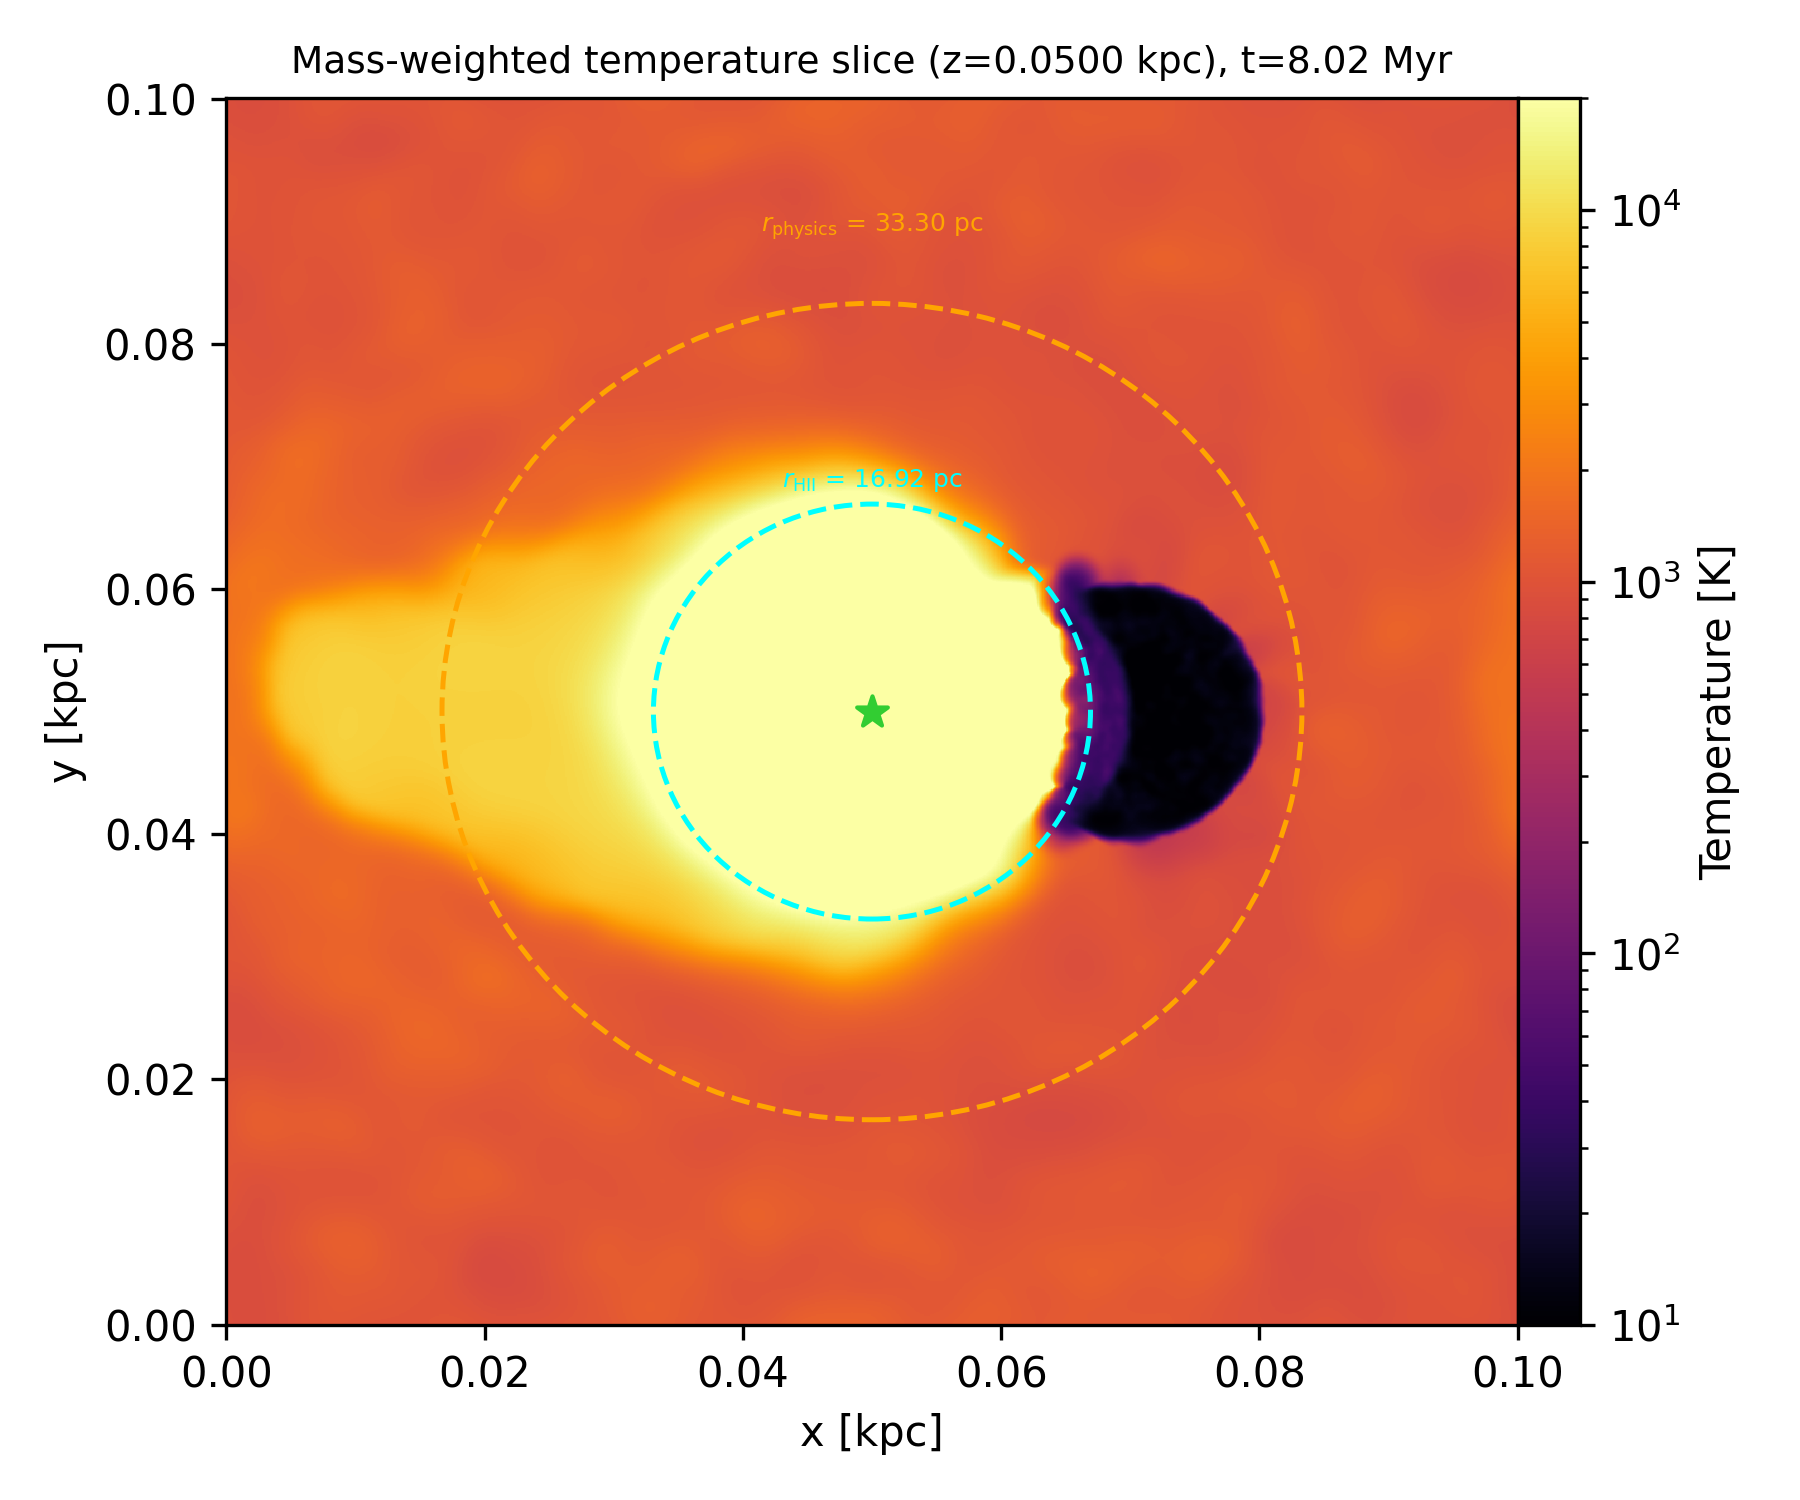
\includegraphics[width=0.48\linewidth]{Figures/det0_freq0p01_uniform_slice}
  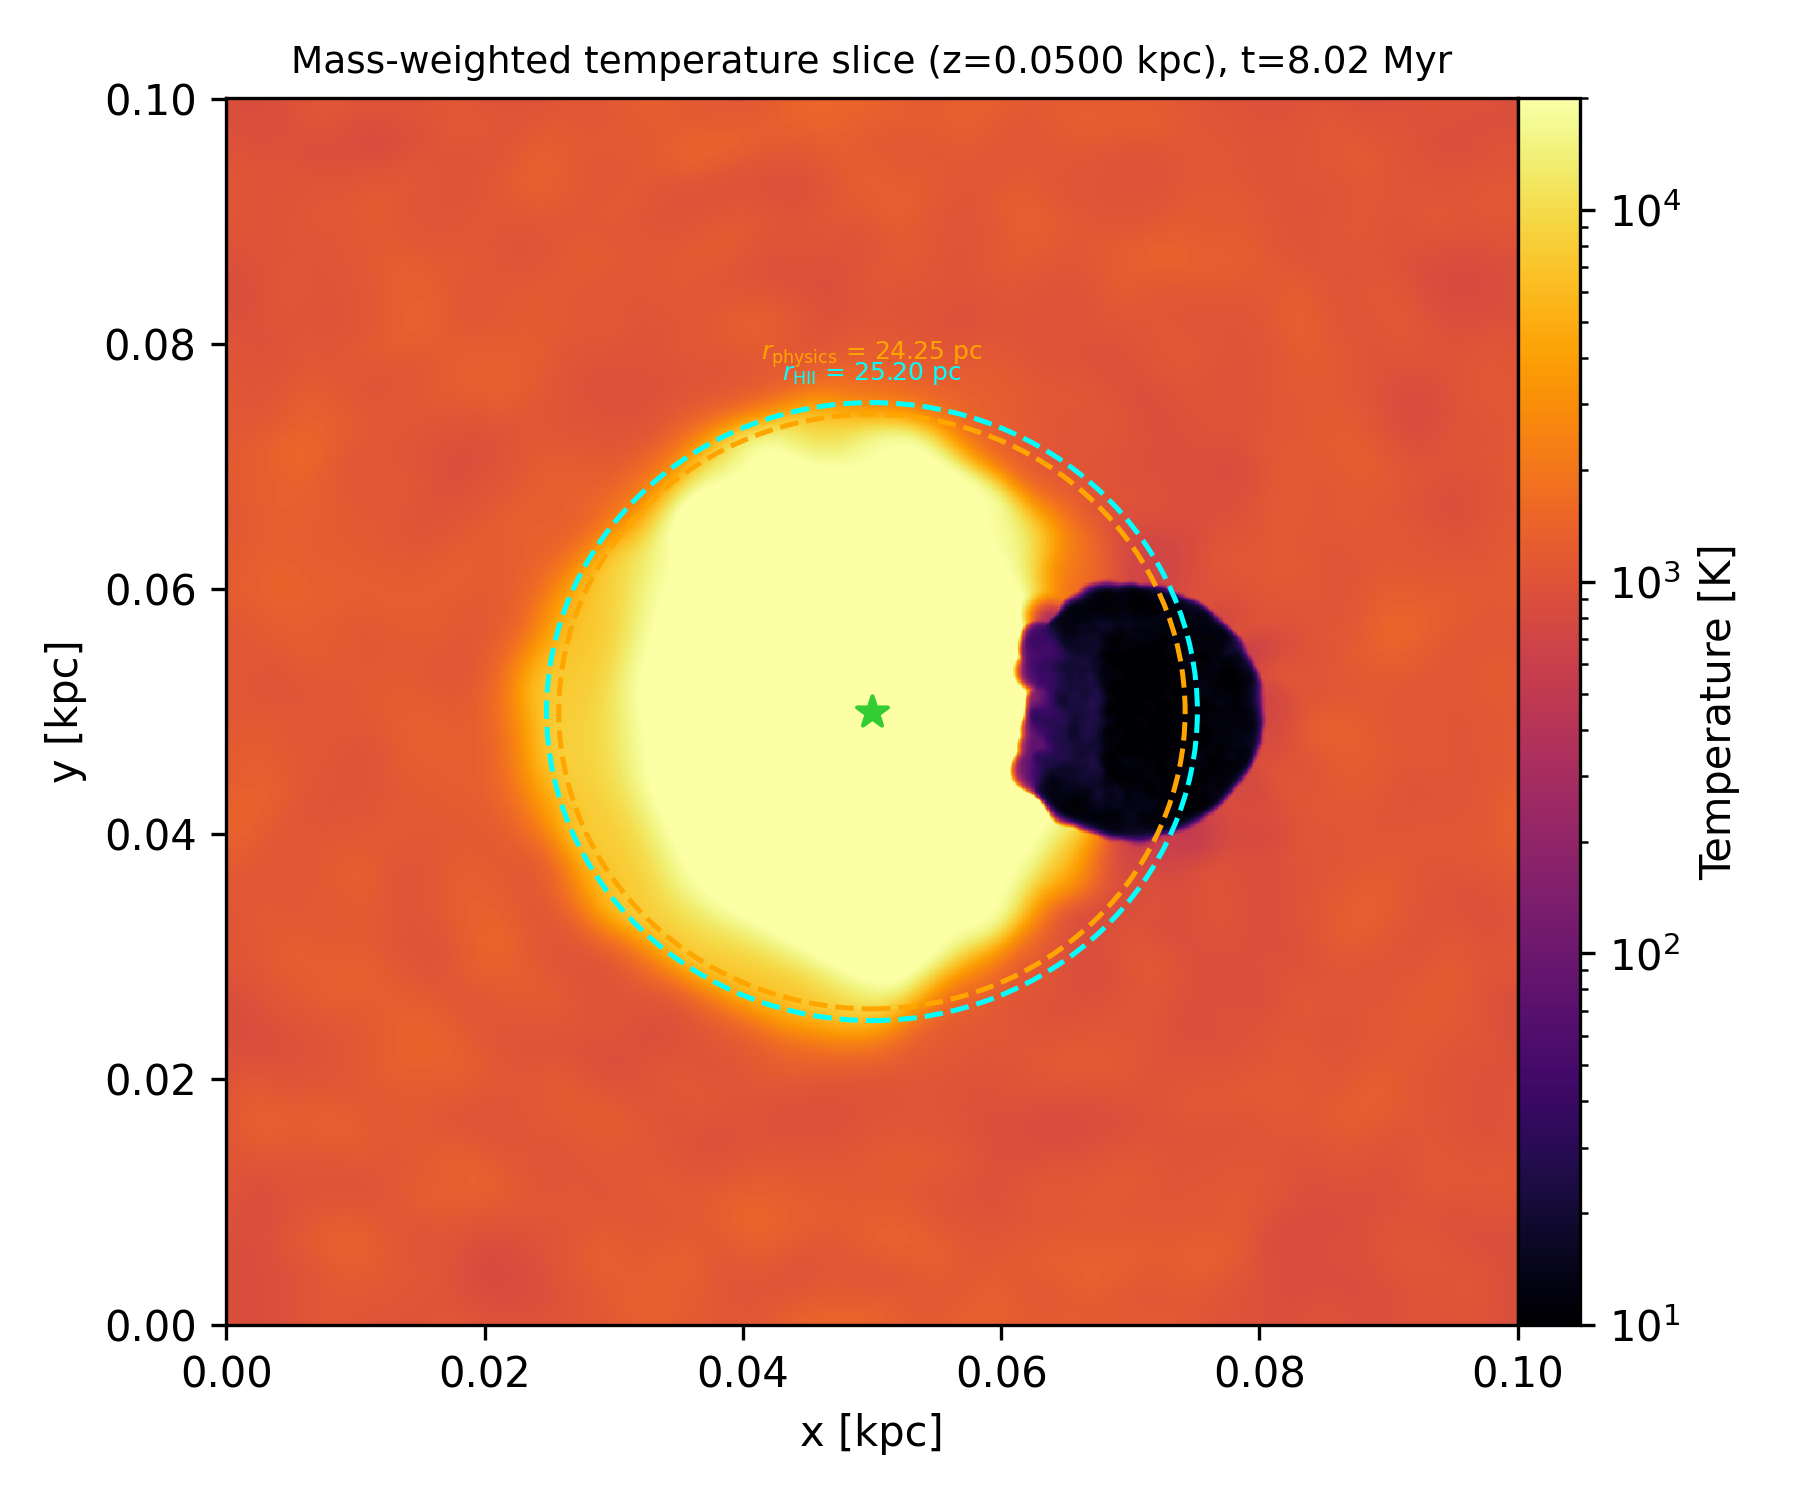
\includegraphics[width=0.48\linewidth]{Figures/det0_freq0p01_angular_slice}
  \caption{Temperature slices at $t=8$\,Myr, probabilistic boundary
    ionization, \texttt{rebuild=0.01\,Myr}. Left: uniform
    (\texttt{nside=0}), $r_{\rm HII}=16.9\,$pc, asymmetric bulge away
    from the clump, clump partially eroded on its star-facing side.
    Right: angular (\texttt{nside=1}), $r_{\rm HII}=25.2\,$pc,
    symmetric, clump intact. Cyan circle: $r_{\rm HII}$ (the
    algorithm's own bookkeeping). Orange circle: $r_{\rm physics}$
    (largest radius to any gas particle with $T>10^4\,$K, regardless
    of tag status).}
  \label{fig:uniform-vs-angular}
\end{figure}

\textbf{$r_{\rm HII}$ can understate the true thermally-affected
extent.} Previously-tagged gas can stay warm well past its tag's
expiry without being re-tagged (low post-evacuation density means a
long local cooling time), so the algorithm's own bookkeeping radius is
a lower bound, not the true extent -- e.g.\ row 1's $r_{\rm
HII}=17.6\,$pc corresponds to $r_{\rm physics}=34.4\,$pc for the same
snapshot. \texttt{plot\_temperature\_hii.py} computes and plots both.

\textbf{The uniform scheme's shortfall relative to the papers is real
but the clump erosion is qualitatively present, not absent.} Checking
temperature by radial shell (not just the deep clump core) at
\texttt{gas\_mass=20}, \texttt{rebuild=0.1}, deterministic, uniform:
the clump's star-facing outer skin (10--13\,pc from the star) reaches
$\sim$28,000\,K, while its shallow interior (13--17\,pc) and core
(17--22\,pc) stay cold ($\lesssim$30--600\,K mean) -- real but shallow
erosion (a few pc deep), not yet the more substantial disruption
\citeauthor{Smith2021} show by 8\,Myr for their spherical scheme.

\textbf{Their idealized-test box is smaller than ours.} Direct
inspection of \citeauthor{Smith2021}'s actual Fig.~2 image (not just
the text) against its 50\,pc scale bar suggests a box in the 60--80\,pc
range, versus our 100\,pc default. This mainly matters for row 2/6
above (getting close to our own half-width); it does not obviously
explain the uniform-scheme shortfall, since a bigger box cannot shrink
an ionized region.
